%; whizzy chapter -dvi
% -initex iniptex -latex platex -format platex -bibtex jbibtex -fmt fmt
% 以上 whizzytex を使用する場合の設定。
 
%     Tokyo Debian Meeting resources
%     Copyright (C) 2012 Junichi Uekawa
%     Copyright (C) 2011, 2015 Nobuhiro Iwamatsu

%     This program is free software; you can redistribute it and/or modify
%     it under the terms of the GNU General Public License as published by
%     the Free Software Foundation; either version 2 of the License, or
%     (at your option) any later version.

%     This program is distributed in the hope that it will be useful,
%     but WITHOUT ANY WARRANTY; without even the implied warranty of
%     MERCHANTABILITY or FITNESS FOR A PARTICULAR PURPOSE.  See the
%     GNU General Public License for more details.

%     You should have received a copy of the GNU General Public License
%     along with this program; if not, write to the Free Software
%     Foundation, Inc., 51 Franklin St, Fifth Floor, Boston, MA  02110-1301 USA

%  preview (shell-command (concat "evince " (replace-regexp-in-string "tex$" "pdf"(buffer-file-name)) "&"))

%%ここからヘッダ開始。

\documentclass[mingoth,a4paper]{jsarticle}
\usepackage{monthlyreport}
% 日付を定義する、毎月変わります。
\newcommand{\debmtgyear}{2016}
\newcommand{\debmtgmonth}{9}
\newcommand{\debmtgdate}{17}
% started from zero:
% (let ((year 2013) (month 7)) (+ (* (- year 2005) 12) month -1))
\newcommand{\debmtgnumber}{143}

\begin{document}

\begin{titlepage}
\thispagestyle{empty}
% タイトルページ:編集必要な部分は最初のマクロに飛ばすこと

\vspace*{-2cm}
第\debmtgnumber{}回 東京エリア Debian 勉強会資料\\
\hspace*{-2cm}

\includegraphics{image2012-natsu/dotdeb.pdf}\\
\hfill{}\debmtgyear{}年\debmtgmonth{}月\debmtgdate{}日

% ここはアップデートすること
% 全角文字にしないとフォントのサイズが合わないので注意
\rotatebox{10}{\fontsize{30}{30} {\gt 特集 :DEP5 再考}}\\

\vspace*{-2cm}
\hfill{}
\includegraphics[height=6cm]{image200502/openlogo-nd.eps}
\end{titlepage}

\newpage

\begin{minipage}[b]{0.2\hsize}
 \definecolor{titleback}{gray}{0.9}
 \colorbox{titleback}{\rotatebox{90}{\fontsize{80}{80} {\gt デビアン勉強会} }}
\end{minipage}
\begin{minipage}[b]{0.8\hsize}
\hrule
\vspace{2mm}
\hrule
\begin{multicols}{2}
\tableofcontents
\end{multicols}
\vspace{2mm}
\hrule
\end{minipage}

\dancersection{最近のDebian関連のミーティング報告}{杉本 典充}

\subsection{第142回東京エリアDebian勉強会}

2016年8月20日(土)に第142回東京エリアDebian勉強会を開催しました。会場は銀座にある朝日ネットさんをお借りして行いました。参加者は6名でした。発表は、dictossさんによる「Debianでlxcをセットアップしてみよう」、飛び込みでkhibinoさんの「haskell-relational-recordの紹介」でした。

dictossさんの「Debianでlxcをセットアップしてみよう」ではlxcのセットアップの手順、lxcの使用例を挙げ、lxc-attachコマンドといったセットアップに便利なコマンドがあるなどディスカッションを行いました。

khibinoさんの「haskell-relational-recordの紹介」では、Haskellにおける集合のプログラミング記法がRDBMSのSQLと親和性の高いことに着目し、Haskellのプログラムをコンパイルする時にはRDBMSのスキーマとの整合性のチェックし、実行時にはSQLを出力してRDBMSとデータをやり取りできるライブラリの紹介がありました。

勉強会終了後は参加者で懇親会を行いました。


\dancersection{事前課題}{杉本 典充}

今回の事前課題は以下です:
\begin{enumerate}
  \item Hack Timeは何をしますか。
\end{enumerate}
この課題に対して提出いただいた内容は以下です。
\begin{multicols}{2}
{\small
\begin{prework}{ 山下康成 }
  \begin{enumerate}
  \item 本日のHackTime作業
  \end{enumerate}
\end{prework}

\begin{prework}{ dictoss }
  \begin{enumerate}
  \item 本日のHackTime作業
  \end{enumerate}
\end{prework}

\begin{prework}{ NOKUBI Takatsugu }
  \begin{enumerate}
  \item 本日のHackTime作業
  \end{enumerate}
\end{prework}

\begin{prework}{ issei }
  \begin{enumerate}
  \item 本日のHackTime作業
  \end{enumerate}
\end{prework}

\begin{prework}{ iwamatsu }
  \begin{enumerate}
  \item 本日のHackTime作業
  \end{enumerate}
\end{prework}

\begin{prework}{ yy\_y\_ja\_jp }
  \begin{enumerate}
  \item 本日のHackTime作業
  \end{enumerate}
\end{prework}

\begin{prework}{ yosuke\_san }
  \begin{enumerate}
  \item 本日のHackTime作業
  \end{enumerate}
\end{prework}

}
\end{multicols}

\dancersection{Debian Trivia Quiz}{杉本 典充}

Debianの昨今の話題についてのQuizです。

今回の出題範囲は\url{debian-devel-announce@lists.debian.org} や \url{debian-news@lists.debian.org}に投稿された内容などからです。

\begin{multicols}{2}
%; whizzy-master ../debianmeetingresume201311.tex
% $B0J>e$N@_Dj$r$7$F$$$k$?$a!"$3$N%U%!%$%k$G(B M-x whizzytex $B$9$k$H!"(Bwhizzytex$B$,MxMQ$G$-$^$9!#(B
%

\santaku
{debain$B%Q%C%1!<%8$N%=!<%9%3!<%I$r%@%&%s%m!<%I$9$kJ}K!$O$"$k$+<ALd$,$"$j$^$7$?!#(BDD$B$NJ}$?$A$,0FFb$7$?%5!<%S%9$O$I$l$G$7$g$&$+!#(B}
{srcs.debian.org}
{srcs.debian.net}
{sources.debian.net}
{C}
{$B4Z9q$G>pJs9)3X$r3X$s$G$$$kBg3X1!@8$NJ}$+$i%;%-%e%j%F%#$N8&5f$N0l4D$GA4%=!<%9%3!<%I$,$[$7$$$H$N$3$H$G$7$?!#$=$N$[$+$K(Bdebmirror$B%3%^%s%I$r;H$&$H$h$$$H$$$&%"%I%P%$%9$b$"$j$^$7$?!#>pJs85(B:\url{https://lists.debian.org/debian-devel/2016/09/msg00118.html}}

\end{multicols}


% % (query-replace-regexp "<.*?>" "")
% % (query-replace-regexp "^[	 ]\+" "")

%-------------------------------------------------------------------------------
\dancersection{DEP5/Machine-readable debian/copyright 再考}{岩松 信洋}
%-------------------------------------------------------------------------------

\subsection{はじめに}

Debian ソースパッケージには debian/copyright ファイルがあり、このファイルには
対象ソフトウェアのライセンス、コピーライトが書かれています。
2009年以前は特にフォーマットもなく、ライセンスも包括的な書き方でした。
例えば gcc-defaults ソースパッケージの debian/copyright ファイルは図
\ref{fig:non-dep5-copyright}のようになっています。

\begin{figure}[htbp]
\begin{center}
\begin{commandline}
gcc-defaults is Copyright (C) 2000, 2001, 2006, 2009 Debian.

These scripts are free software; you can redistribute it and/or modify it
under the terms of the GNU General Public License as published by the
Free Software Foundation; either version 2, or (at your option) any
later version.

On Debian GNU/Linux systems, the complete text of the GNU General
Public License can be found in `/usr/share/common-licenses/GPL'.

The c89 and c99 man pages are taken from netbsd:

Copyright (c) 1999 The NetBSD Foundation, Inc.
All rights reserved.
(省略)
\end{commandline}
\end{center}
\caption{DEP5 非準拠な debian/copyright}
\label{fig:non-dep5-copyright}
\end{figure}


2010年頃 Debian開発者であるSteve Langasek らによって debian/copyright ファイルを
機械処理できるフォーマットに切り替え、自動チェックなどができるようにするため、
DEP5 / Machine-readable debian/copyright (以下、DEP5)が策定されました(\url{http://dep.debian.net/deps/dep5/})。
策定後 BTS 609160 によって Debian Policy に取り込まれ、Debian Policy の一部(Debian Policy 12.5、オプショナル扱い)
となっています。最新バージョンは 1.0 であり、最新版は
\url{https://www.debian.org/doc/packaging-manuals/copyright-format/1.0/}
から参照できます。

策定から6年近く経ち、多くのパッケージがDEP5 準拠の debian/copyright 
になっています。しかしこのファイル、Debian Policy でもオプショナル扱いという
こともあり、一度作ってしまうとあまり更新しないということもあり、内容が変更され
ずそのまま続けるという問題もあります。
今回は DEP5 についてのフォーマットの紹介と、debian/copyright ファイルの更新方法について
紹介します。

\subsection{DEP5 フォーマットについて}

DEP5のフォーマットはヘッダー部とファイル部で分けられます。
ヘッダー部にはソフトウェア全体に関わる情報、例えば頒布元や連絡先、
ファイル部にはファイル毎のコピーライトとライセンスを記述します。

ヘッダー部で利用できるフィールドは以下の通りです。
\begin{itemize}

  \item Format:

        フォーマット内容が書かれたファイルのURIを指定します。
        実際には\url{https://www.debian.org/doc/packaging-manuals/copyright-format/1.0/}を指定します。
        昔はpackaging-manualsに含まれていなかったため、議論の場であった wikiのURI
        (\url{http://wiki.debian.org/Proposals/CopyrightFormat})や\texttt{http://} が指定されている
        パッケージもあります。

  \item Upstream-Name:

        アップストリームのソフトウェアパッケージ名を指定します。Debianの場合は実際のソフトウェア名とDebianソース
        パッケージ名が異なる場合があります。このフィールドはオプション扱いです。

  \item Upstream-Contact:

        アップストリームの連絡先を指定します。このフィールドはオプション扱いです。

  \item Source:

        ソース頒布先を指定します。このフィールドはオプション扱いです。

  \item  Disclaimer:

        ソフトウェアの免責事項を記載します。contrib や non-freeのパッケージの場合に利用します。このフィールドはオプション扱いです。

  \item  Comment:

        コメントを記載します。ソフトウェアのライセンスが複雑な経緯を持っている場合などに利用される
        ようです。このフィールドはオプション扱いです。

  \item  License:

         ライセンスを記載します。最初の行ではライセンスのショートバージョンを指定し、
         次の行からはローカルファイルシステムにあるライセンスファイルへのパス(
         例:/usr/share/common-licenses/GPL-2)と、ソフトウェア保証の放棄や問題が
         あった場合の通知方法などを含めた文章を記載します。
         もしライセンスファイルがローカルファイルシステムにない場合は全文記載す
         る必要があります。
         ショートバージョンのライセンスの記載方法ですが、GNU GPL version2 or later の場合は\texttt{GPL-2+}、
         Creative Commons Attribution Share Alike license 3.0の場合は\texttt{CC-BY-SA-3.0}と指定する
         ことができます。
         詳細は\url{https://www.debian.org/doc/packaging-manuals/copyright-format/1.0/#license-short-name}を参照してください。
         このフィールドはオプション扱いです。

  \item  Copyright:

         コピーライトホルダーを記載します。このフィールドはオプション扱いです。

\end{itemize}

上記のフォーマットだけでは、ファイル毎にライセンスが異なる場合、記載することが難
しくなります。なので、本フォーマットでは、上記に加え、ファイル毎のライセンスとコ
ピーライトホルダーを記載するファイル部のフォーマットがあります。
ファイル部で利用できるフィールドは以下の通りです。
\begin{itemize}
  \item  Files:

         ファイルを記載します。同じライセンス、コピーライトホルダーをもつファイ
         ルをまとめて記載することができます。
  \item  Copyright:

         コピーライトホルダーを記載します。
  \item  License:

         ライセンスを記載します。記載方法は上記の方法と同じです。ライセンスは同
         じだが、ファイル毎にコピーライトホルダーが異なる場合、ラインセンスのシ
         ョートバージョンのみを記載し、本文をまとめて記載することもできます。
         例を図\ref{fig:repeat-license}に示します。

\begin{figure}[htbp]
\begin{center}
\begin{commandline}
Files: *
Copyright: foo bar <foo@example.org>
License: GPL-2+

Files: debian/*
Copyright: Nobuhiro Iwamatsu <iwamatsu@debian.org>
License: GPL-2+
 This program is free software; you can redistribute it
 and/or modify it under the terms of the GNU General Public
 License as published by the Free Software Foundation; either
 version 2 of the License, or (at your option) any later
 version.
 .
 This program is distributed in the hope that it will be
 useful, but WITHOUT ANY WARRANTY; without even the implied
 warranty of MERCHANTABILITY or FITNESS FOR A PARTICULAR
 PURPOSE.  See the GNU General Public License for more
 details.
 .
 You should have received a copy of the GNU General Public
 License along with this package; if not, write to the Free
 Software Foundation, Inc., 51 Franklin St, Fifth Floor,
 Boston, MA  02110-1301 USA
 .
 On Debian systems, the full text of the GNU General Public
 License version 2 can be found in the file
 `/usr/share/common-licenses/GPL-2'.
\end{commandline}
\end{center}
\caption{ライセンスの繰り返し例}
\label{fig:repeat-license}
\end{figure}


  \item  Comment:

         コメントを記載します。このフィールドはオプション扱いです。
\end{itemize}

上記を組み合わせることによって debian/copyright ファイルを DEP5 準拠に
します。

その他、擬似フィールドとして ライセンスの許諾情報を記載する License-Grant フィールド、
ラインセスファイルへのパスを記載する License-Reference フィールドを使っている
場合もあります(\debianbug{786450})。

\subsection{DEP5 の問題点と対策}

上記で説明したフォーマットを定義した DEP5 ですが、ファイルが多くなるほど記載する
ことが難しくなり、あまり更新されないという問題があります。また DEP5 はポリシーで
もオプショナルなので、移行があまり進んでいないという問題もあります。

ここでは debian/copyright の DEP5 化と更新方法について紹介します。

\subsubsection{licensecheck を使ったDEP5 フォーマット化}

指定したディレクトリにあるファイルのライセンスとコピーライトホルダーを出力する
licensecheck というツールがあります(図\ref{fig:licensecheck})。
これは昔は devscripts で提供されていましたが、分離され(\debianbug{828872})、licensecheck パッケージで
提供されるようになりました。
\texttt{-r} オプションで指定したディレクトリを再帰的に検索、\texttt{--copyright} オプショ
ンでコピーライトホルダーを出力するようにします。
実行例を図\ref{fig:licensecheck}に示します。

\begin{figure}[htbp]
\begin{center}
\begin{commandline}
$ licensecheck -r --copyright .
ell/io.h: LGPL (v2.1 or later)
  [Copyright: 2011-2014 Intel Corporation. All rights reserved]

ell/dbus.c: LGPL (v2.1 or later)
  [Copyright: 2011-2014 Intel Corporation. All rights reserved]
(省略)
\end{commandline}
\end{center}
\caption{licensecheckコマンド実行例}
\label{fig:licensecheck}
\end{figure}

これだけでは DEP5 フォーマットにならないため、cdbsで提供されている
/usr/lib/cdbs/licensecheck2dep5 を使って整形します(図
\ref{fig:update-copyright-by-cdbs})。

\begin{figure}[htbp]
\begin{center}
\begin{commandline}
$ licensecheck -r --copyright .  | /usr/lib/cdbs/licensecheck2dep5

Format: http://www.debian.org/doc/packaging-manuals/copyright-format/1.0/
Upstream-Name: FIXME
Upstream-Contact: FIXME
Source: FIXME
Disclaimer: Autogenerated by CDBS

Files: ./ell/base64.c
 ./ell/base64.h
 ./ell/checksum.c
 (中略) 
 ./unit/test-uuid.c
Copyright: 2011-2014, Intel Corporation.
  2011-2015, Intel Corporation.
  2011-2016, Intel Corporation.
  2015, Intel Corporation.
  2016, Intel Corporation.
License: LGPL (v2.1 or later)
 FIXME
(省略) 
\end{commandline}
\end{center}
\caption{licensecheck2dep5 による debian/copyright 更新方法}
\label{fig:update-copyright-by-cdbs}
\end{figure}

DEP5フォーマットにして出力してくれますが、License フィールドが\texttt{FIXME}
になっていたり、ASCII 以外の文字は文字化けするなど、完璧な出力はしてくれないため、
生成されたテキストを修正する必要があります。

\subsubsection{cme を使った DEP5 フォーマット化と debian/copyright の更新}

licensecheck2dep5 より少し賢い出力をしてくれるツールとして cme があります。
これは汎用的な設定ファイル編集ツールなのですが、libconfig-model-dpkg-perl パッケ
ージ をインストールすることにより、debian パッケージ用のモデルが使えるようになります。
debian/copyright を更新したい場合には \texttt{dpkg-copyright} オプションを使います。
実行するとDEP5 フォーマットで debian/copyright に出力します(図\ref{fig:update-copyright})。
\footnote{cme は "cme check dpkg-control" といった debian/control に対するチェックなども
行えます。この話はまた今度。}

\begin{figure}[htbp]
\begin{center}
\begin{commandline}
$ sudo apt-get install cme libconfig-model-dpkg-perl
$ cme update dpkg-copyright
cme: using Dpkg::Copyright model
updating data
(省略)
\end{commandline}
\end{center}
\caption{CME による debian/copyright 更新方法}
\label{fig:update-copyright}
\end{figure}

またlibconfig-model-tkui-perl パッケージをインストールするとGUIで編集できるようなり
ます(図\ref{fig:edit-copyright}、図\ref{fig:cme-gui})。

\begin{figure}[htbp]
 \begin{minipage}{0.5\hsize}
\begin{center}
\begin{commandline}
$ sudo apt-get install libconfig-model-tkui-perl
debian/copyright を編集したい場合
$ cme edit dpkg-copyright
debian/copyright を更新した後、編集したい場合
$ cme update dpkg-copyright --edit
エディタで直接編集でも大丈夫です。
$ cme update dpkg-copyright
$ vi debian/copyright
\end{commandline}
\end{center}
\caption{debian/copyright 編集方法}
\label{fig:edit-copyright}
 \end{minipage}
 \begin{minipage}{0.5\hsize}
\begin{center}
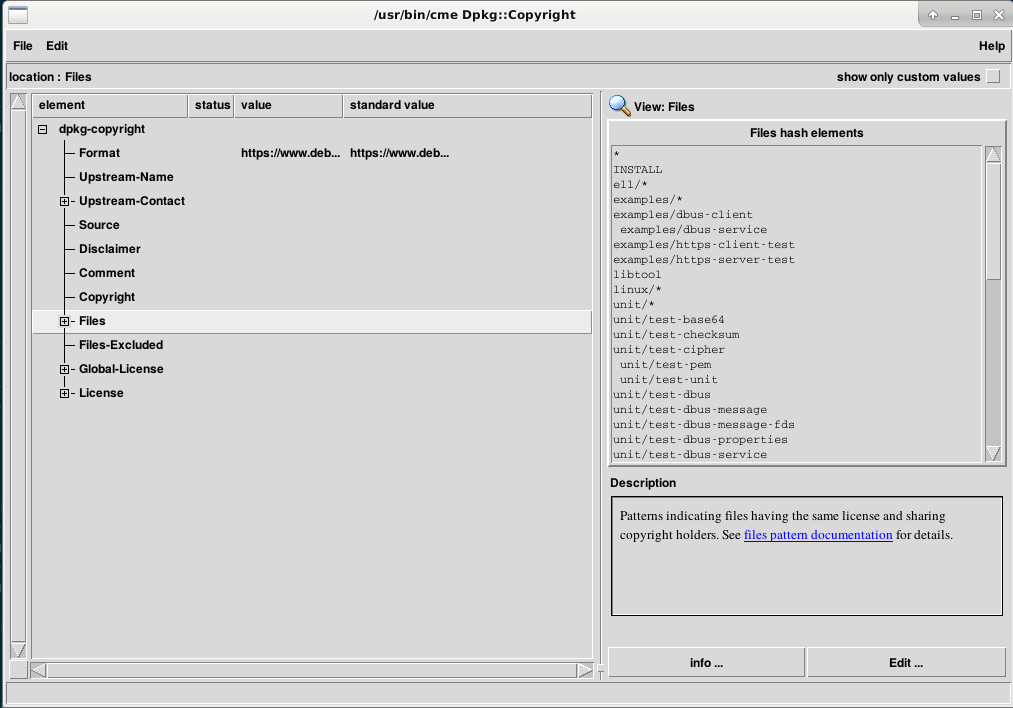
\includegraphics[width=0.7\hsize]{image201609/cme-gui.png}
\end{center}
\caption{cme GUI起動画面}
\label{fig:cme-gui}
 \end{minipage}
\end{figure}

これもlicensecheck2dep5と同様、完璧な出力はしてくれないため、出力
された debian/copyright ファイルを確認して修正する必要があります。
またUTF-8に対応しているため、ASCII文字以外でも正しく処理してくれます。

\subsubsection{debmake を使った debian/copyright の DEP5フォーマット化}

debmake コマンドの \texttt{-cc} オプションを使ってDEP5フォーマット化された
debian/copyright を作成することもできます。

\begin{commandline}
$ debmake -cc > debian/copyright
\end{commandline}

cme との違いは ファイルを列挙する点(cmeはワイルドカード($\ast$)でまとめる)
と 不要なファイル(例 debian/copyright)の内容まで確認してしまうなどがあります。
debmake は ソースパッケージ作成サポートツールなので、更新機能がまだないのだと
思います。個人的には今のところ debian ディレクトリ以下のファイルチェックにも
使える cme をお薦めします。

\subsubsection{license-reconcile による debian/copyright チェックサポート}


license-reconcile を使うことによって、
cme などで捕捉できないファイルのライセンスやコピーライトが debian/copyright が書かれているか、チェック
できるようにするツールとして\texttt{license-reconcile} があります。
これは\texttt{license-reconcile}パッケージによって提供されています。
例えば、今まで全てのファイルが\texttt{GPL-3+}でライセンスされていたプログラム
(図\ref{fig:example-copyright})に
\texttt{GPL-2+}でライセンスされている\texttt{hoge.png} ファイルが取り込まれた
とします。バイナリファイルなので cme などでは検知できません。

\begin{figure}[htbp]
\begin{center}
\begin{commandline}
Files: *
Copyright: 2016 foo bar <foo@example.org>
License: GPL-3+
\end{commandline}
\end{center}
\caption{debian/copyright 例}
\label{fig:example-copyright}
\end{figure}

debian/copyright に記載されているかチェックできるようにするため、
\texttt{debian/license-reconcile.yml} ファイルを用意し、図
\ref{fig:example-license-reconcile}のような内容を記述します。

\begin{figure}[htbp]
\begin{center}
\begin{commandline}
Rules:
 rules:
  -
   Glob: hoge.png
   License: GPL-2+
   Copyright: 2016 foo bar <foo@example.org>
\end{commandline}
\end{center}
\caption{debian/license-reconcile.yml 例}
\label{fig:example-license-reconcile}
\end{figure}

\texttt{license-reconcile}コマンド を実行すると以下のようなコピーライトミスマッチエラー
が出力されます(図\ref{fig:example-license-reconcile})。

\begin{figure}[htbp]
\begin{center}
\begin{commandline}
$ license-reconcile
License mismatch: File hoge.png has license GPL-2+ which does not match GPL-3+.\
at /usr/share/perl5/Debian/LicenseReconcile/App.pm line 222, <GEN0> line 3.
\end{commandline}
\end{center}
\caption{license-reconcile 実行例}
\label{fig:example-license-reconcile}
\end{figure}

debian/copyright に \texttt{hoge.png} に関するフィールド(図
\ref{fig:example-update-copyright})を追加し、再度
\texttt{license-reconcile} コマンドを実行するとラインセンスフィールドチェックエラーが
出力されなくなります。

\begin{figure}[htbp]
\begin{center}
\begin{commandline}
Files: hoge.png
Copyright: foo bar <foo@example.org>
License: GPL-2+
 This program is free software: you can redistribute it and/or modify
 it under the terms of the GNU General Public License as published by
 the Free Software Foundation, either version 2 of the License, or
 (at your option) any later version.
(省略)
\end{commandline}
\end{center}
\caption{debian/copyright 追記例}
\label{fig:example-update-copyright}
\end{figure}

\subsubsection{debian パッケージ側の対応}

上記では licensecheck や cme といった ツールを使うことによって debian/copyright ファイルを
DEP5 フォーマットに切り替えることができることを説明しましたが、debian/rules にチ
ェック用のターゲットを追加することのよって、パッケージのメンテナンス性が向上しま
す。図\ref{fig:example-update-rules} のように debian/rules へ追記し
\texttt{debian/rules update-debian-copyright}を実行することにより、DEP 5 フォー
マット の debian/copyright を debian/copyright.auto に出力します。

\begin{figure}[htbp]
\begin{center}
\begin{commandline}
# cme を使う場合
update-debian-copyright:
	cme update dpkg-copyright -file debian/copyright.auto
# licensecheck + licensecheck2dep5 を使う場合
update-debian-copyright:
        licensecheck --copyright -r `find * -type f` | \
                /usr/lib/cdbs/licensecheck2dep5 > debian/copyright.auto
\end{commandline}
\end{center}
\caption{debian/rules 追記例}
\label{fig:example-update-rules}
\end{figure}

\subsection{まとめ}

DEP5 フォーマットの簡単な内容紹介と、debian/copyright の DEP5 フォーマットするた
めのツールの使い方、debian パッケージでの利用方法について説明しました。
以下、まとめです。
\begin{itemize}
\item DEP 5 は Debian ポリシーの一部。しかしオプショナル扱い。
フォーマット詳細は
\url{https://www.debian.org/doc/packaging-manuals/copyright-format/1.0/}または
\url{/usr/share/doc/debian-policy/copyright-format-1.0.txt.gz}にある。

\item licensecheck ツールによって ソースからのライセンスとコピーライトホルダーを
抽出可能。そのままではDEP5フォーマットにならないため、licensecheck2dep5を使う。
\item cme と libconfig-model-dpkg-perl を使うことによって licensecheck +
licensecheck2dep5 同様のことが可能。岩松のお勧めはこちら。
\item license-reconcile を使うことによって cme などで補完できないファイルのチェ
ックができる。
\item 毎回 cme や licencecheck などのコマンドを実行するのではなく、debian/rules 
に書いておくとメンテナンスが楽になる。
\end{itemize}

%
% 冊子にするために、4の倍数にする必要がある。
% そのための調整
%\dancersection{メモ}{}
\mbox{}\newpage


\vspace*{15cm}
\hrule
\vspace{2mm}

\includegraphics[width=2cm]{image200502/openlogo-nd.eps}
\noindent \Large \bf Debian 勉強会資料\\
\noindent \normalfont \debmtgyear{}年\debmtgmonth{}月\debmtgdate{}日 \hspace{5mm}  初版第1刷発行\\
\noindent \normalfont 東京エリア Debian 勉強会 (編集・印刷・発行)\\
\hrule

\end{document}
